\documentclass{article}
\usepackage[utf8]{inputenc}
\usepackage{amsmath}
\usepackage{amsfonts}
\usepackage{subcaption}
\usepackage{multirow}
\usepackage{siunitx}
\usepackage{parskip}
\usepackage{marvosym}
\usepackage{mathtools}
\usepackage{graphicx} % Include figure files
\usepackage{bm}
\usepackage{booktabs}
\usepackage{hyperref}
\usepackage{pdfpages}
\usepackage[T1]{fontenc}
\usepackage{baskervillef}
\usepackage[varqu,varl,var0]{inconsolata}
\usepackage[scale=.95,type1]{cabin}
\usepackage[baskerville,vvarbb]{newtxmath}
\usepackage[cal=boondoxo]{mathalfa}
\usepackage{natbib}
\usepackage{graphicx}
\usepackage{librebaskerville}
\usepackage[T1]{fontenc}
\usepackage{float}
\usepackage{xcolor}
\title{Instrumentation Amplifier}
\author{Amaan Rahman \\
The Cooper Union \\
ECE-444: Bio-instrumentation}

\begin{document}
\maketitle
%===== ABSTRACT =====%
\section{Abstract}
The instrumentation amplifier is 2-stage amplifier; the former stage consists of 2 differential operation amplifiers configured as buffer amplifiers, and the latter stage consists of a unity gain amplifier. The advantages of this amplifier topology are high open loop gain and high Common-Mode-Rejection-Ratio (CMMR). Thus, the instrumentation amplifier is practical in scenarios where a differential signal is small and further amplification is required. 

%===== INTRODUCTION =====%
\section{Introduction}
\begin{figure}[h!]
    \begin{center}
        \fbox{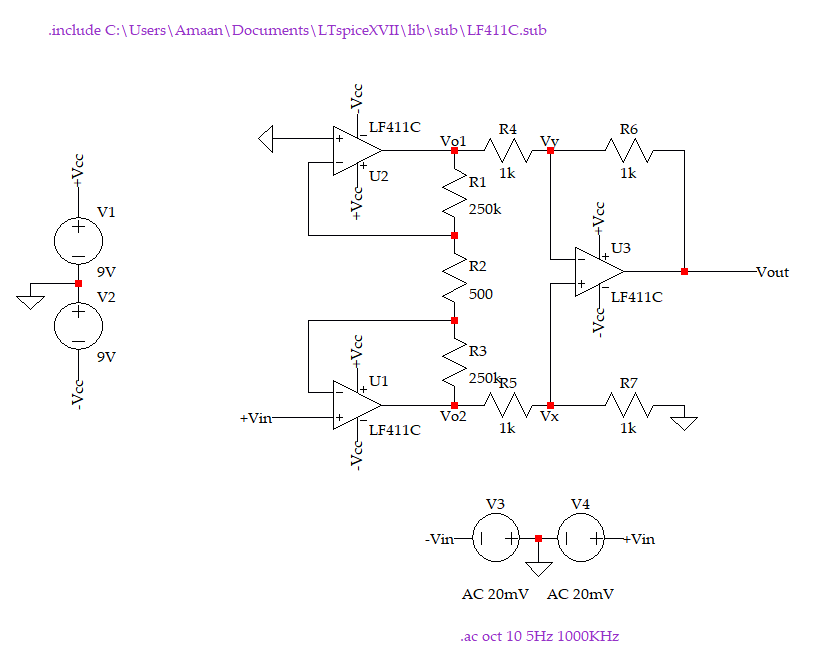
\includegraphics[scale=0.5]{simulation/spice_schematic.png}}
    \end{center}
    \caption{LTSpiceVII instruementation amplifier schematic}
    \label{fig:spice-schematic}
\end{figure}

An LTSpice simulation schematic has been setup, as can be seen in \textbf{Figure~\ref{fig:spice-schematic}}. The physical circuit has been built accordingly to the topology structure in \textbf{Figure~\ref{fig:circuit-setup}}. \\

Let $v_{o_i}$ represent the output voltages of each respective operational amplifier, and $v_x,\;v_y$ be the input volatges of the unity gain buffer. \\ 

According to the proof of the instrumentation amplifier (\textit{in-amp}) voltage gain, it can be seen that the output voltage is equivalent to the differential input of the output stage of the \textit{in-amp}:
\[
    \begin{rcases}
        \frac{v_{out} - v_y}{R} =& \frac{v_y - v_{o_1}}{R} \\
        \frac{v_{out} - v_x}{R} =& \frac{v_{o_2} - v_x}{R}
    \end{rcases} \implies v_{out} = v_{o_2} - v_{o_1} \because \{v_x = v_y\}
\]
Thus, the final stage is a unity gain buffer due to having a voltage gain of 1. 

The differential input of the \textit{in-amp} can be expressed as so: 
\begin{equation*}
    \Delta v_{in} = v_{+in} - v_{-in} \\
\end{equation*}
Given the gain of the output stage, the gain of the \textit{in-amp} can be derived by applying basic node analysis on the input stage:
\begin{equation*}
    \begin{aligned}
        \frac{v_{o_2} - v_{o_1}}{2R_2 + R_1} &= \frac{\Delta v_{in}}{R_1} \\
        \frac{v_{out}}{2R_2 + R_1} &= \frac{\Delta v_{in}}{R_1} \\
        A_v = \frac{v_{out}}{v_{in}} &= 1 + \frac{2R_2}{R_1}
    \end{aligned}
\end{equation*}

%===== PROCEDURE =====%
\section{Procedure}
\begin{figure}[h!]
    \begin{center}
        \fbox{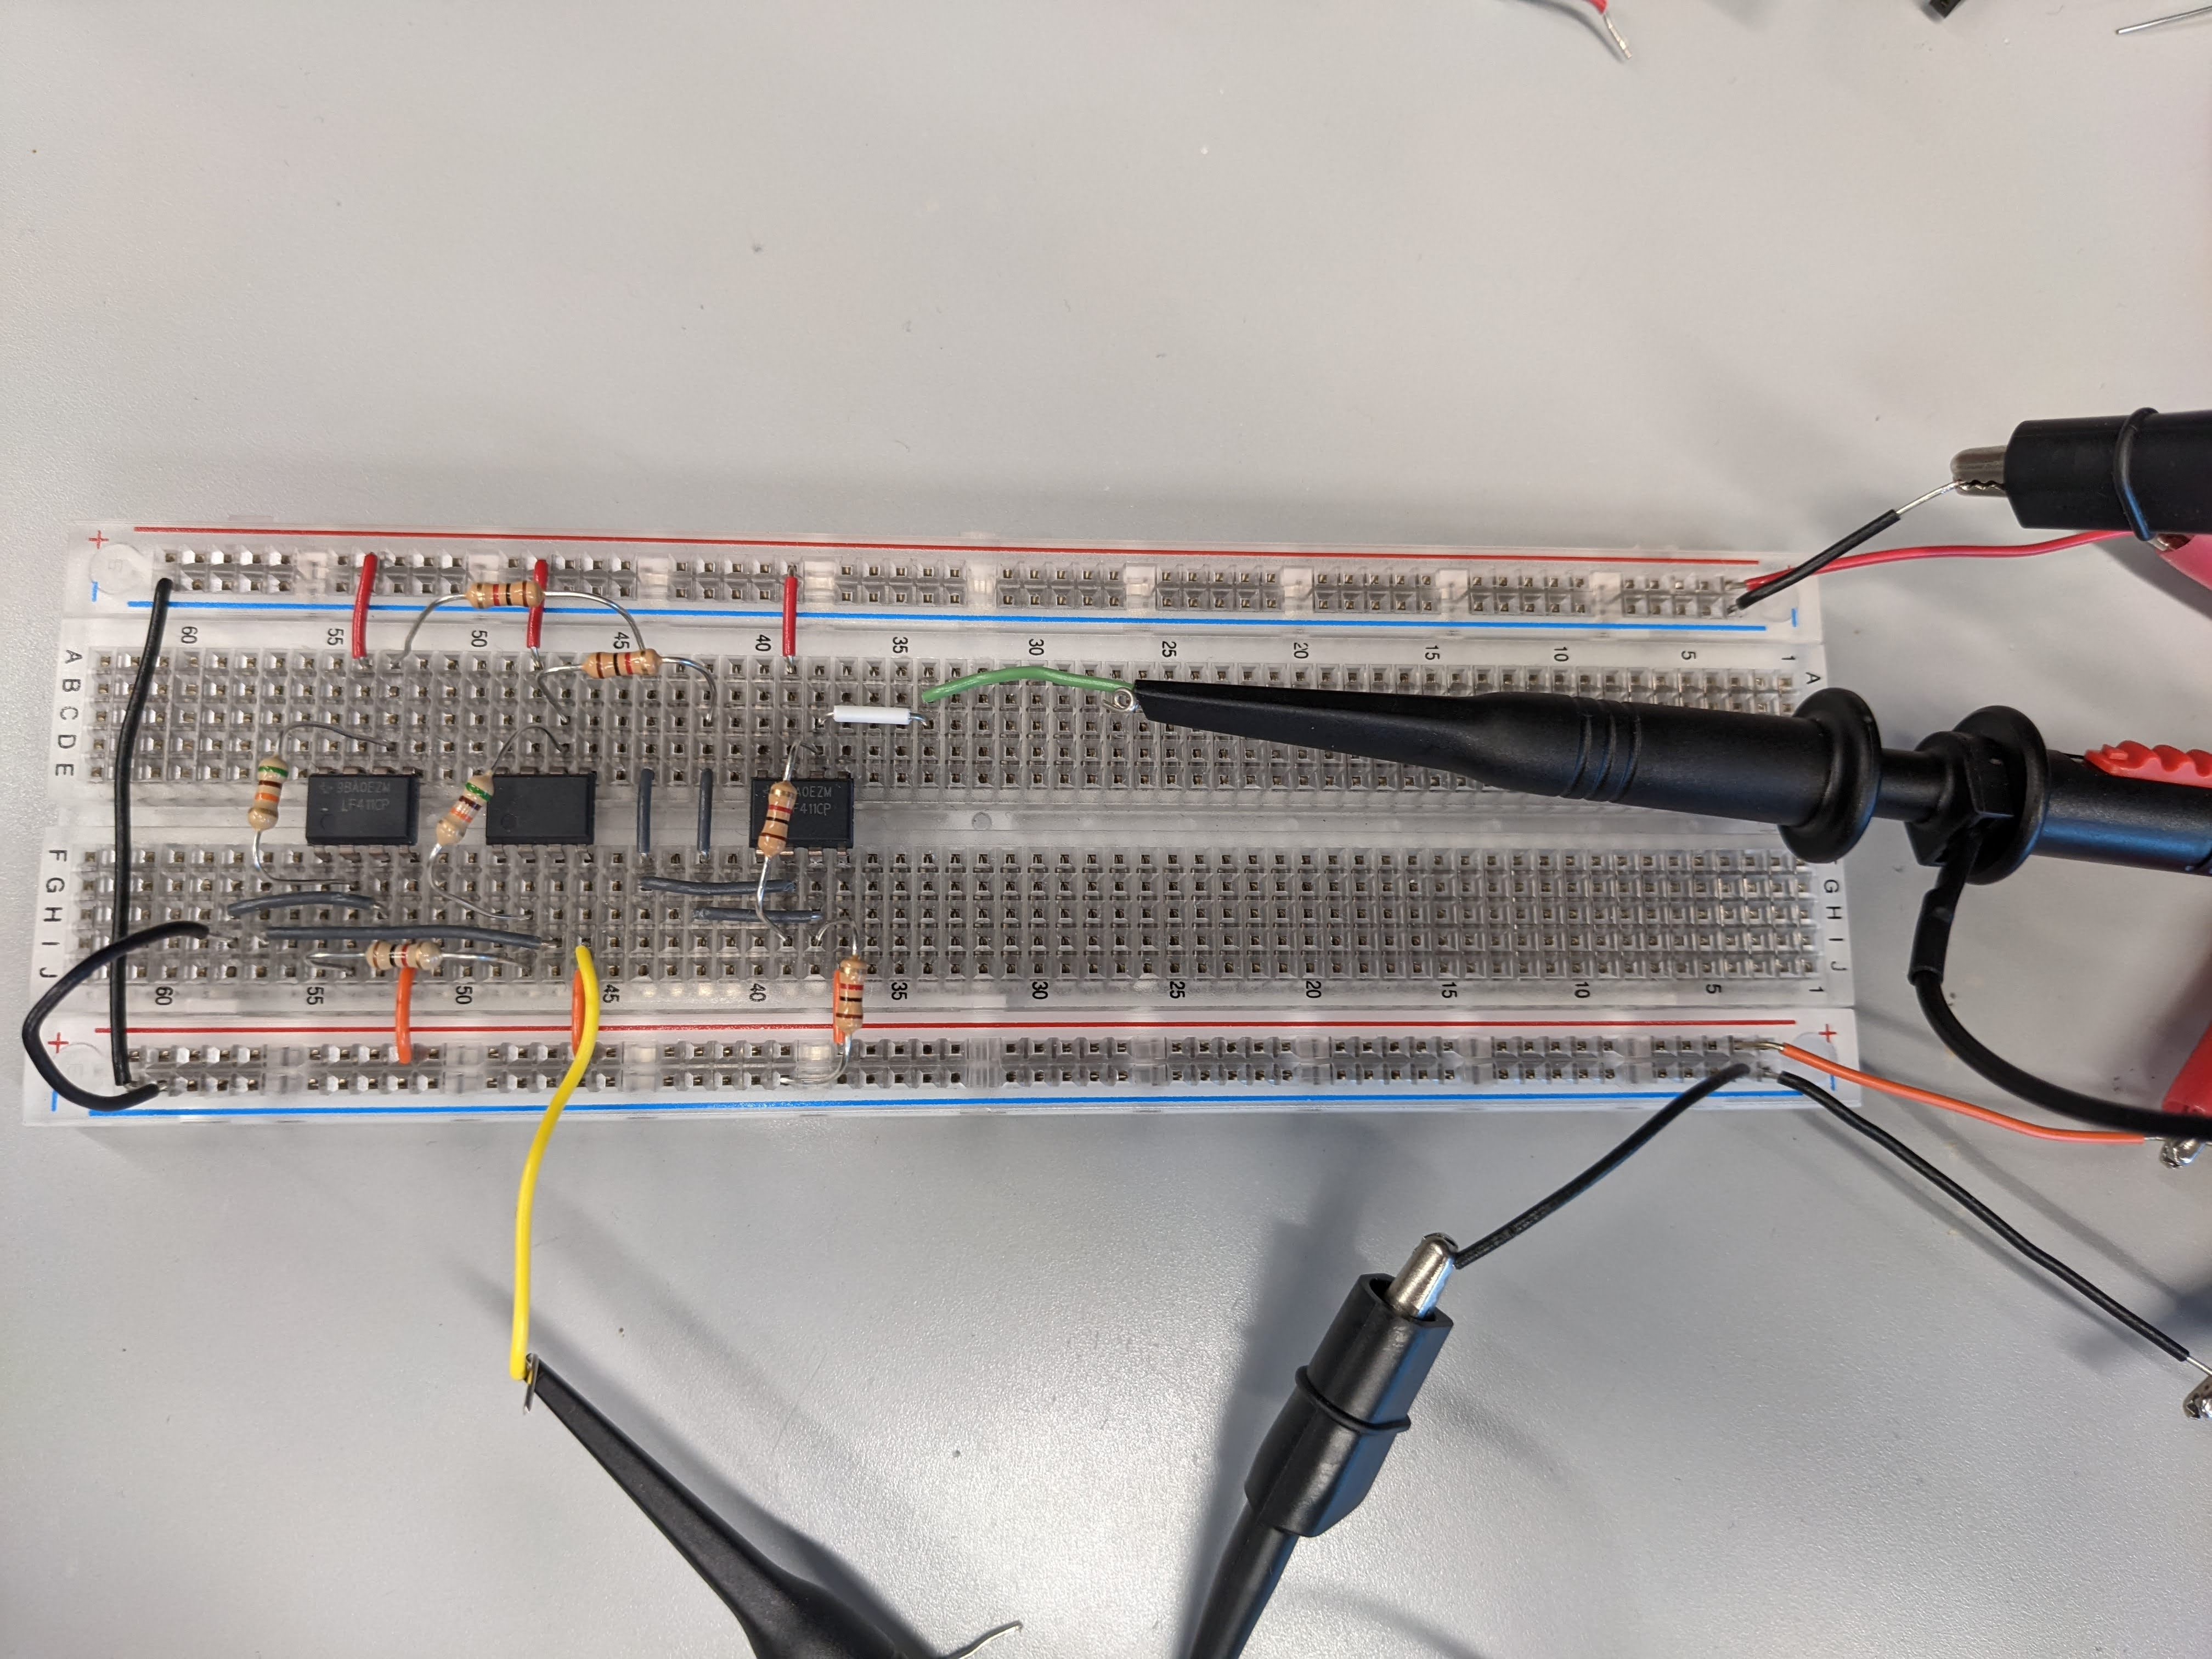
\includegraphics[scale=0.08]{simulation/circuit_setup.jpg}}
    \end{center}
    \caption{Breadboard layout of instrumentation amplifier. From left to right, the first 2 411s make up the input stage and the last 411 is the output stage. \textcolor{red}{Red} wire implies $+Vcc$, \textcolor{orange}{orange} wire implies $-Vcc$, \textbf{black} wire implies ground, \textcolor{yellow}{yellow} wire implies probe conenction to oscilloscope input \textbf{1}, \textcolor{green}{green} wire implies probe connection to oscilloscope input \textbf{2}, \textcolor{gray}{gray} wire implies diffierntial input to operational amplifier, and \textit{white} wire implies output of intrumentation amplifier.}
    \label{fig:circuit-setup}
\end{figure}

Components: 
\begin{itemize}
    \item 3 411 Operational amplifiers
    \item $R_2:\;250k\Omega$
    \item $R_1:\;500\Omega$
    \item $R:\;1k\Omega$
\end{itemize}

The (-) terminal of the \textit{in-amp} is grounded and the (+) terminal is connected to an oscilloscope wave generator. The frequency response was plotted in courtesy of Richard Lee's script to automate gain data collection for a range of frequencies sweeped from 1Hz to 7kHz. The Common Mode Rejection Ratio (CMMR) was determined by dividin the differential gain by the common mode gain at a specifc frequency, 1kHz in this case. Power dissipation of each operational amplifier was determined for a detailed analysis.
%===== RESULTS =====%
\section{Results}
\subsection{Frequency Response}
\begin{figure}[H]
    \begin{center}
        \fbox{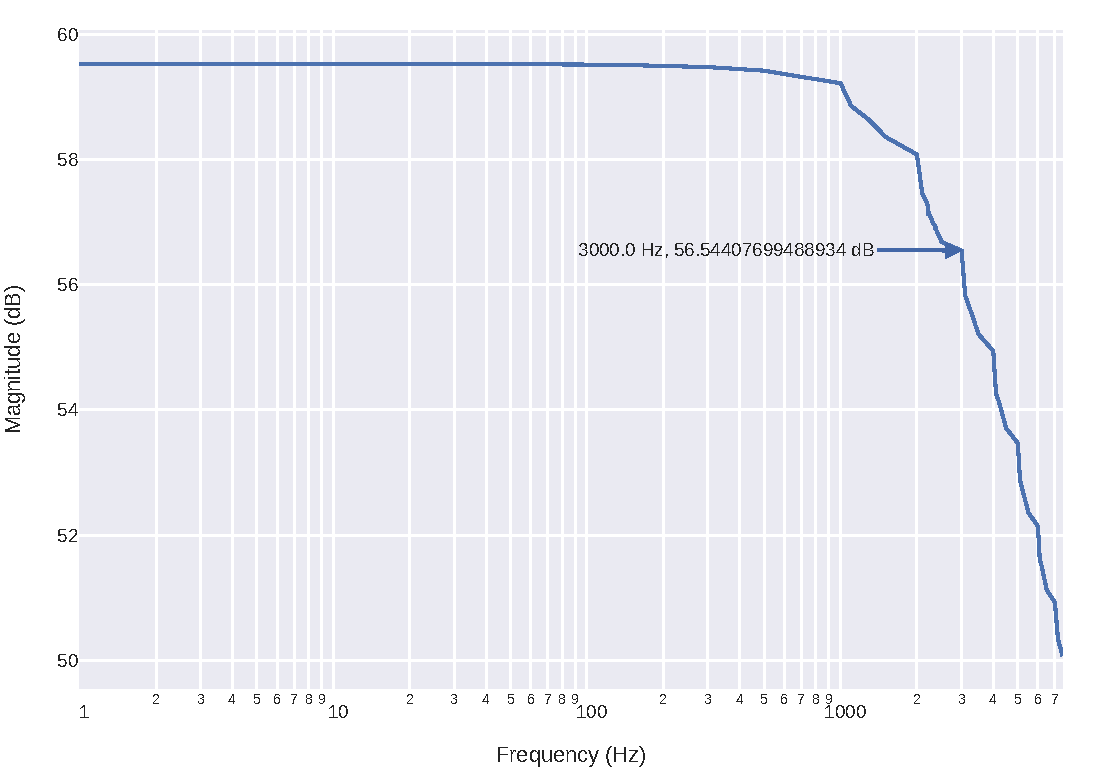
\includegraphics[scale=0.5]{simulation/frequency_response_a.pdf}}
    \end{center}
    \caption{Frequency response of instrumentation amplifier. Corner frequency not accurately depicted due to delays in capturing gain data for every sweep interval towrads the end. Gain is approximately 60dB between 1Hz and 1kHz.}
    \label{fig:gain-plot}
\end{figure}
\subsection{CMMR}
\begin{equation*}
    \begin{aligned}
        V_{CM_{out}} =& 16mV \\
        V_{CM_{in}}  =& 1.2mV \\
        A_{CM} =& \frac{16mV}{1.2V} = 0.0133
    \end{aligned}
\end{equation*}
\newline
\begin{equation*}
    \begin{aligned}
        V_{diff_{out}} =& 37mV \\
        V_{diff_{in}}  =& 42mV \\
        A_{diff} =& \frac{37V}{42mV} = 880.952
    \end{aligned}
\end{equation*}
\newline
\begin{equation*}
    CMMR = \frac{A_{diff}}{A_{CM}} = 66236.992
\end{equation*}

\subsection{Power Dissipation}


%===== DISCUSSION =====%
\section{Discussion}
According to \textbf{Figure~\ref{fig:gain-plot}}, the corner frequency is around 2kHz; however, in simulation, \textbf{Figure~\ref{fig:sim-gain-plot}}, the corner frequency is around 1kHz. This ~1kHz difference in the corner frequency could be due to the propogated delays of capturing the gain at each frequency in the frequency response through a script to automate the frequency response, in courtesy of Richard Lee. It could also be due to the resistance values and the effect of parasitic capacitances of the operational amplifier. 

There was difficulty in figuring out where the corner frequency is derived from exactly, but through prolonged experimentation and simulations, manipulating $R_2$ and $R_1$ ratio such that gain is very large ($\sim500\,\frac{V}{V}$) yields in decreasing the corner frequency such that the bandwidth decreases dramatically. 

Another difficulty was generating the frequency response of the instrumentation amplifier without tabulating oscciliscope data by hand.  Due to never using a spectrum analyzer before, it took time to figure it out. Nonetheless, all signals were visible at various frequencies. If the center frequency matches the frequency of the output signal frequency, a main lobe is oberseved with a gain (dB) that matches the expected gain of the intrumentation amplifier. However, a frequency sweep was required to generate the approprite gain bode plot of the instrumentation amplifier, and that functionality could not be discovered as of yet.
\section{Appendix: Simulations}
\begin{figure}[h!]
    \begin{center}
        \fbox{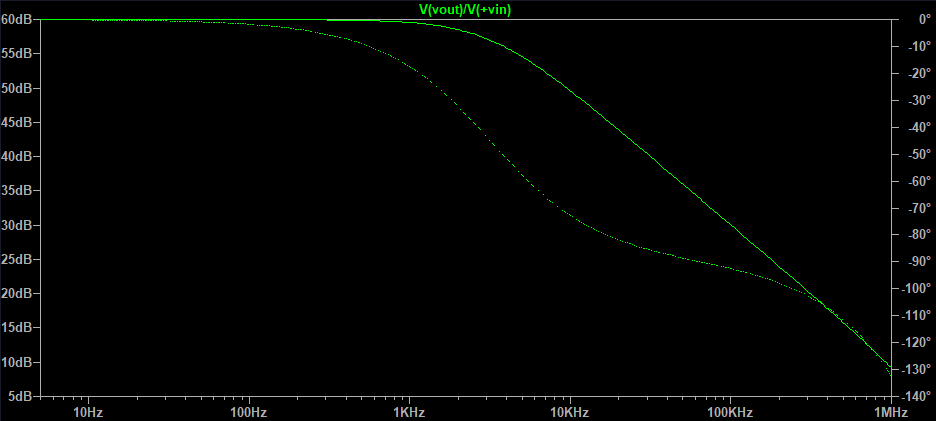
\includegraphics[scale=0.65]{simulation/bode_plot_right.png}}
    \end{center}
    \caption{LTSpiceVII frequency response simulation 5Hz-1MHz AC sweep 20mV.}
    \label{fig:sim-gain-plot}
\end{figure}
\end{document}

